\chapter{Dezvoltarea aplicației web}
   În acest capitol, conceptele teoretice prezentate anterior și algoritmii de multicolorare implementați sunt integrați într-o aplicație practică: o aplicație web care permite utilizatorilor să își planifice joburile, utilizând tehnici de multicolorare a grafurilor pentru optimizarea alocării resurselor și a timpului.

\section{Arhitectura generală a aplicației}
  Aplicația creată pornește de la arhitectura clasică MERN (acronim provenit de la cele patru componente principale: MongoDB, Express.js, React.js, Node.js), extinsă prin integrarea algoritmilor descriși în capitolul~\ref{cap:algoritmi}, implementați în Python.

\begin{figure}[h]
\centering
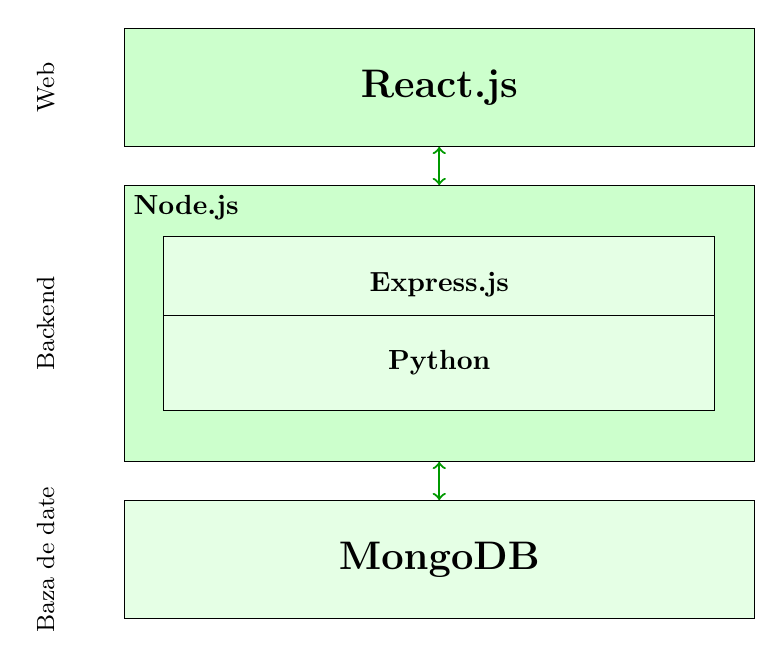
\begin{tikzpicture}[
    box/.style={rectangle, draw, minimum width=8cm, minimum height=1.5cm, align=center, font=\Large\bfseries},
    container/.style={rectangle, draw, minimum width=8cm, minimum height=3.5cm, align=center, font=\Large\bfseries, fill=green!20},
    innerbox/.style={rectangle, draw, minimum width=7cm, minimum height=1.2cm, align=center, font=\normalsize\bfseries, fill=green!10},
    layer/.style={font=\small, rotate=90, anchor=center},
    arrow/.style={<->, thick, green!60!black}
]

\node[layer] at (-1, 6) {Web};
\node[layer] at (-1, 3) {Backend};
\node[layer] at (-1, 0) {Baza de date};

\node[box, fill=green!20] (react) at (4, 6) {React.js};


\node[container] (server) at (4, 3) {};
\node[innerbox] (express) at (4, 3.5) {Express.js};
\node[innerbox] (python) at (4, 2.5) {Python};
\node[anchor=north west] at (server.north west) {\bfseries Node.js};

\node[box, fill=green!10] (mongo) at (4, 0) {MongoDB};

\draw[arrow] (react.south) -- (server.north);
\draw[arrow] (server.south) -- (mongo.north);

\end{tikzpicture}
\caption{Arhitectura aplicației web}\label{fig:arhitectura}
\end{figure}

O să analizăm figura~\ref{fig:arhitectura} pornind de jos în sus.

{\bf Baza de date MongoDB}

MongoDB este o bază de date NoSQL (neralațională), flexibilitatea ei permite o stocare eficientă a datelor necesare planificării joburilor. Astfel prin intermediul ei se stochează:
\begin{itemize}
  \item informațiile despre utilizatori (cu date de autentificare și profil),
  \item datele despre planificarea joburilor (parametrii necesari precum numărul de resurse partajate, detalii despre joburi, incompabilitățile)
  \item rezultatele algoritmilor de planificare
\end{itemize}
Biblioteca folosită pentru interacțiunea cu baza de date, simplificând operațiile CRUD este \textit{Mongoose}.

{\bf Backend Node.js}

Node.js a fost ales ca mediu de execuție pentru backend datorită simplității și a ecosistemului bogat de pachete NPM, care susține dezvoltarea rapidă de funcționalități pentru planificarea și gestionarea joburilor Utilizarea JavaScript pe ambele părți (frontend și backend) reduce complexitatea dezvoltării și facilitează întreținerea codului.
Express.js completează această alegere ca framework web minimalist, oferind structura necesară pentru API-urile RESTful care gestionează operațiile de planificare, monitorizare și control al job-urilor. 
Dependențele cheie utilizate în backend sunt:
\begin{itemize}
  \item \textit{bcrypt.js} pentru hash-uirea și securizarea parolelor utilizatorilor.
  \item \textit{child\_process} vital pentru aplicația noastră deorece permite rularea proceselor externe cum ar fi scripturile Python care implementează algoritmii de multicolorare.
  \item \textit{jsonwebtoken și cookie-parser}: Pentru implementarea autentificării bazate pe token-uri JWT și gestionarea sesiunilor utilizatorilor.
  \item \textit{cors}: Middleware care permite comunicarea între frontend și backend când sunt pe domenii diferite.
\end{itemize}

{\bf Web React.js}

React.js a fost ales pentru dezvoltarea interfeței utilizator (UI) deoarece arhitectura sa bazată pe componente permite construirea unor interfețe complexe și interactive într-un mod organizat și scalabil. În contextul unei aplicații de planificare a joburilor, unde utilizatorii interacționează cu grafuri și trebuie să vizualizeze și să modifice datele, utilizarea React.js facilitează implementarea unor elemente UI dinamice și oferă o experiență de utilizare fluidă și intuitivă.
Dependențele ce merită menționate sunt:
\begin{itemize}
  \item \textit{axios} pentru cereri HTTP asincrone către backend.
  \item \textit{html-to-image} permite generare unui imagini (în cazul nostru, PNG) dintr-un element HTML. Este folosită pentru a permite utilizatorilor să exporte rezultate sub formă de imagine.
  \item \textit{papaparse} permite parsarea unui fisier CSV în JavaScript. Este utilizată pentru a permite utilizatorilor să importe date despre planificarea dorită.
  \item \textit{reactflow} $-$ biblioteca de bază pentru aplicația construită. Prin intermediul ei se realizează și se vizualizează grafurile ce reprezintă planficarea utilizatorului.
\end{itemize}


\section{ Prelucrarea și introducerea datelor în aplicație}
\subsection{Modelul datelor în backend și legătura cu problema planificării}

Pentru a reprezenta modelul teoretic al grafului de incompabilitate și al parametrilor asociați (prezentați în capitolul~\ref{cap:multicolorare}), datele sunt stocate în baza de date MongoDB folosind schema următoare:
\begin{itemize}
  \item \textit{Joburile V} sunt modelate prin obiecte în lista jobs, fiecare având câmpurile: processing\_time ($p_i$), gain ($g_i$).
  \item Muchiile de incompabilitate \textit{E} sunt reprezentate în lista conflicts, fiecare conflict indicând două joburi incompatibile.
  \item Parametrii globali precum deadline-ul D și numărul de resurse l sunt stocați ca atribute directe ale planificării.
\end{itemize} 

\vspace{2cm}
\begin{lstlisting}[language=JavaScript, caption={Schema modelului de date pentru planificare}, label={Schedule}]

  const embeddedJobSchema = new mongoose.Schema({
  _id: { type: String, required: true },
  name: { type: String, required: true },
  processing_time: { type: Number, required: true },
  gain: { type: Number, required: true },
  position: {
    x: { type: Number, required: true },
    y: { type: Number, required: true },
  },
}, { _id: false });

const embeddedConflictSchema = new mongoose.Schema({
  _id: { type: String, required: true },
  job1: { type: String, required: true },
  job2: { type: String, required: true },
}, { _id: false });

const scheduleSchema = new mongoose.Schema({
  userId: { type: mongoose.Schema.Types.ObjectId, 
  ref: "User", required: true },
  name: { type: String, required: true },
  jobs: [embeddedJobSchema],
  conflicts: [embeddedConflictSchema],
  l: { type: Number, required: true },
  D: { type: Number, required: true },
  created_at: { type: Date, default: Date.now },
  updated_at: { type: Date, default: Date.now },
});

const Schedule = mongoose.model("Schedule", scheduleSchema);
export default Schedule;
\end{lstlisting}


\subsection{Modelul pentru stocarea rezultatelor algoritmilor de planificare}

Pentru a salva rezultatele algorimilor prezentați în capitolul~\ref{cap:algoritmi} împreună cu scorurile funcțiilor obiectiv ($f_1$,$f_2$,$f_3$)
astfel încat utilizatorul să poate vizualiza rezultatele, am definit următorul modul Mongoose:

\begin{lstlisting}[language=JavaScript, caption={Schema modelului de date pentru rezultatul planificării},label={ScheduleResult}
]
const scheduleSchemaResultSchema = new mongoose.Schema({
  userId: { type: mongoose.Schema.Types.ObjectId, 
  ref: "User", required: true },
  schemaId: {
    type: mongoose.Schema.Types.ObjectId,
    ref: "Schedule",
    required: true,
  },
  fully_colored_jobs: [{ type: String }],
  color_map: { type: mongoose.Schema.Types.Mixed, 
  default: {} }, 
  f1: { type: Number },
  f2: { type: Number },
  f3: { type: Number },
  algorithm_used: { type: String },
  timestamp: { type: Date, default: Date.now },
});

const ScheduleSchemaResult = mongoose.model(
  "ScheduleSchemaResult",
  scheduleSchemaResultSchema
);
export default ScheduleSchemaResult;
\end{lstlisting}

\subsection{Introducerea datelor}
Acum vom urmări fluxul datelor de la interfeța grafică până la backend, iar apoi la algoritmii de planificare.
Utilizatorul are două metode prin care poate introduce datele despre planificare:
\begin{enumerate}
  \item Manual, prin adaugăre joburilor și trasarea incompabilităților.
  \item Import, prin intermediul unui fișier CSV.\
\end{enumerate}

\begin{figure}[h]
    \centering
    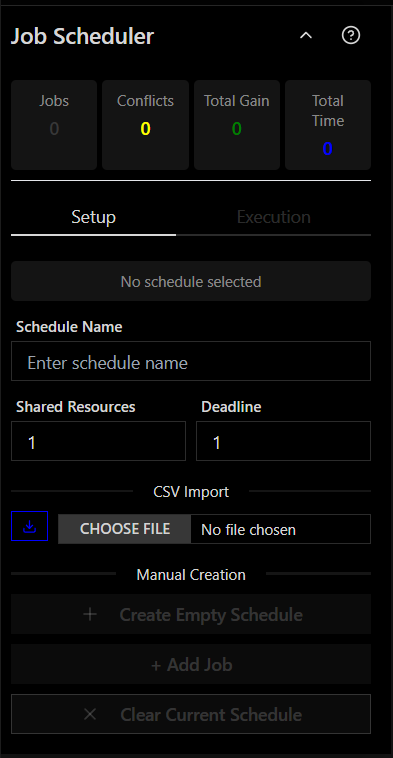
\includegraphics[width=0.5\textwidth]{images/ControlPanel.png}
    \caption{Introducerea datelor}\label{fig:ControlPanel}
\end{figure}

Procesul de introducere a datelor respectă un flux logic pentru a asigura consis- tența și validitatea acestora. În primul rând, utilizatorul trebuie să creeze un nou obiect de planificare (\texttt{Schedule}), fără de care nu se pot adăuga joburi. Odată creat, utilizatorul are la dispoziție două metode pentru a introduce joburi și conflicte: manual (prin interfața grafică) sau prin importul unui fișier CSV.\ Pentru a facilita această operațiune, aplicația permite descărcarea unui template de CSV, iar fișierul importat este supus unei funcții de parsare și validare. În cadrul acestei etape, datele din CSV sunt verificate pentru consistență (de exemplu, nu sunt permise joburi cu nume duplicate), iar utilizatorul poate vizualiza un \textit{preview} al conținutului înainte de salvare. De asemenea, backend-ul implementează reguli stricte de validare a datelor introduse. Această abordare asigură că datele transmise algoritmilor de planificare respectă structura necesară pentru generarea unor rezultate valide.

\subsection{Prelucrarea datelor}
După ce utilizatorul a introdus datele despre planificare (joburi, conflicte și parametri globali), acestea sunt salvate în baza de date prin modelul \textit{Schedule}~\ref{Schedule} iar când utilizatorul dorește generarea unei planificării, backend-ul extrage aceste date și le pregătește într-un format compatibil cu algorimtii implementați în Python. Pe scurt, datele sunt transformate într-un obiect JSON care este trimis prin stdin către un script Python. Acesta preia informațiile și le convertește într-un mod compatibil cu algoritmii. Rezultatul returnat este de asemenea un JSON ce este primit,validat și stocat în \textit{ScheduleSchemaResult}~\ref{ScheduleResult}.Ulterior, rezultatul poate fi vizualizat de către utilizator în interfața grafică și de asemenea descărcat sub formă unei imagini.

\begin{figure}[h]
    \centering
    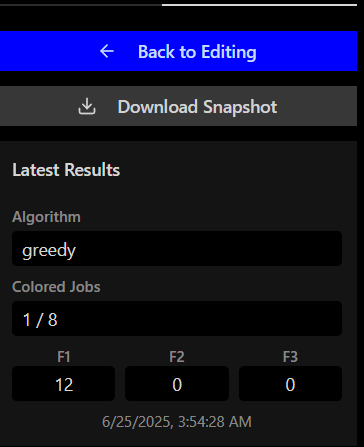
\includegraphics[width=0.5\textwidth]{images/Rezultat.png}
    \caption{Rezultatul unei rulări}\label{fig:Rezultat}
\end{figure}

\section{Modulul de multicolorare și interfața utilizator}

În secțiunea anterioară am prezentat fluxul de introducere și prelucrare a datelor, însă nu am detaliat modul de afișare grafică a joburilor — componentă esențială a interfeței aplicației. Aceasta cuprinde două stări distincte: modul de editare, în care utilizatorul configurează planificarea, și modul de afișare a rezultatului, în care vizualizează soluția generată de algoritmi.

\begin{figure}[h]
\centering
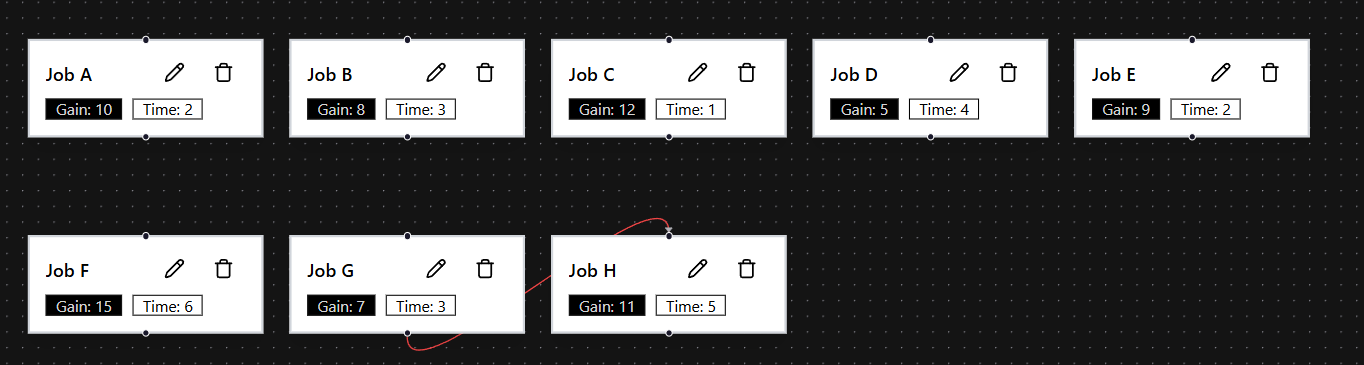
\includegraphics[width=0.9\textwidth]{images/noduri.png}
\caption{Modul de editare al joburilor}\label{fig:noduri}
\end{figure}

În figura~\ref{fig:noduri} este ilustrat modul de editare. În această etapă, utilizatorul poate adăuga și poziționa noduri (joburi), poate trasa muchii de incompatibilitate prin conectarea a două noduri, precum și edita parametrii unui job (timp de procesare, câștig, denumire) sau șterge complet un job existent.

\begin{figure}[h]
\centering
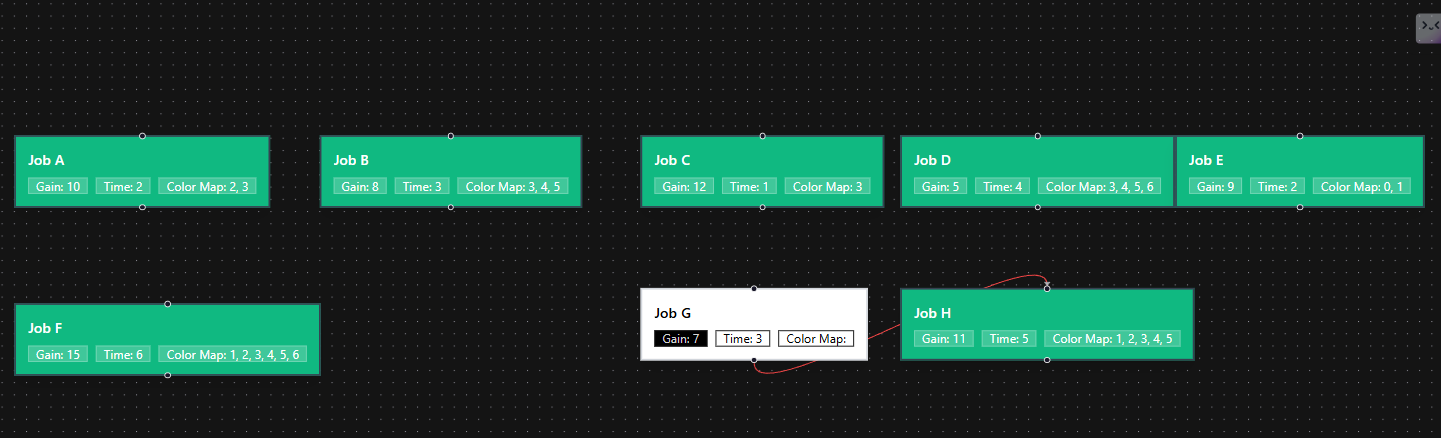
\includegraphics[width=0.9\textwidth]{images/noduri_rezultat.png}
\caption{Afișarea rezultatului algoritmului de multicolorare}\label{fig:noduri_rezultat}
\end{figure}

În figura~\ref{fig:noduri_rezultat} este redat modul de afișare a rezultatului. După rularea unui algoritm de planificare, nodurile colorate complet sunt evidențiate în verde, iar fiecare job afișează culoarea alocată de algoritm, reprezentând resursa la care a fost atribuit.

